\chapter{Foundation}

\section*{Introduction}
This chapter details the implementation phase of our project, which follows an agile methodology with four sprints. Each sprint focuses on delivering specific features and functionality according to the project backlog. The implementation utilizes a modern tech stack consisting of React \cite{ReactWebsite} with Vite \cite{ViteJSWebsite} for the frontend, Node.js \cite{NodeJSWebsite} with Express.js \cite{ExpressJSWebsite} for the backend, MySQL \cite{MySQLWebsite} for database management, and Tailwind CSS \cite{TailwindWebsite} for styling.

Our first sprint focused on establishing essential foundational components of the system, with the following key deliverables:

\subsection{Web Backoffice Authentication}
\begin{itemize}
    \item Admin dashboard login and authentication system
    \item Role-based access control for backoffice users (Super Admin, Admin, Agent)
    \item User management interface for creating and managing user accounts
    \item Permission management system for different user roles
    \item Security logs and audit trails for backoffice activities
    \item Session management and secure token handling
\end{itemize}

\section{Sprint 1: Authentication and User Management }
\subsection{Overview}
The first sprint focuses on establishing the core authentication system and user management functionality. This foundation is critical for all subsequent features as it defines user roles and access controls.

\subsection{User Types}
The system supports three distinct user types, each with different permissions and capabilities:
\begin{itemize}
    \item \textbf{Super Admin}: Has complete access to all system features and can manage admins and agents.
    \item \textbf{Admin}: Can manage agents and has access to administrative features within their assigned scope.
    \item \textbf{Agent}: Has limited access to the system based on their assigned responsibilities.
\end{itemize}


\subsection{Authentication System}
\subsubsection{Sign-up Process}
The sign-up process is illustrated in Figure \ref{fig:signup-diagram} below. The diagram shows the authentication flow for new users registering in the system.

\begin{figure}[ht!]
    \centering
    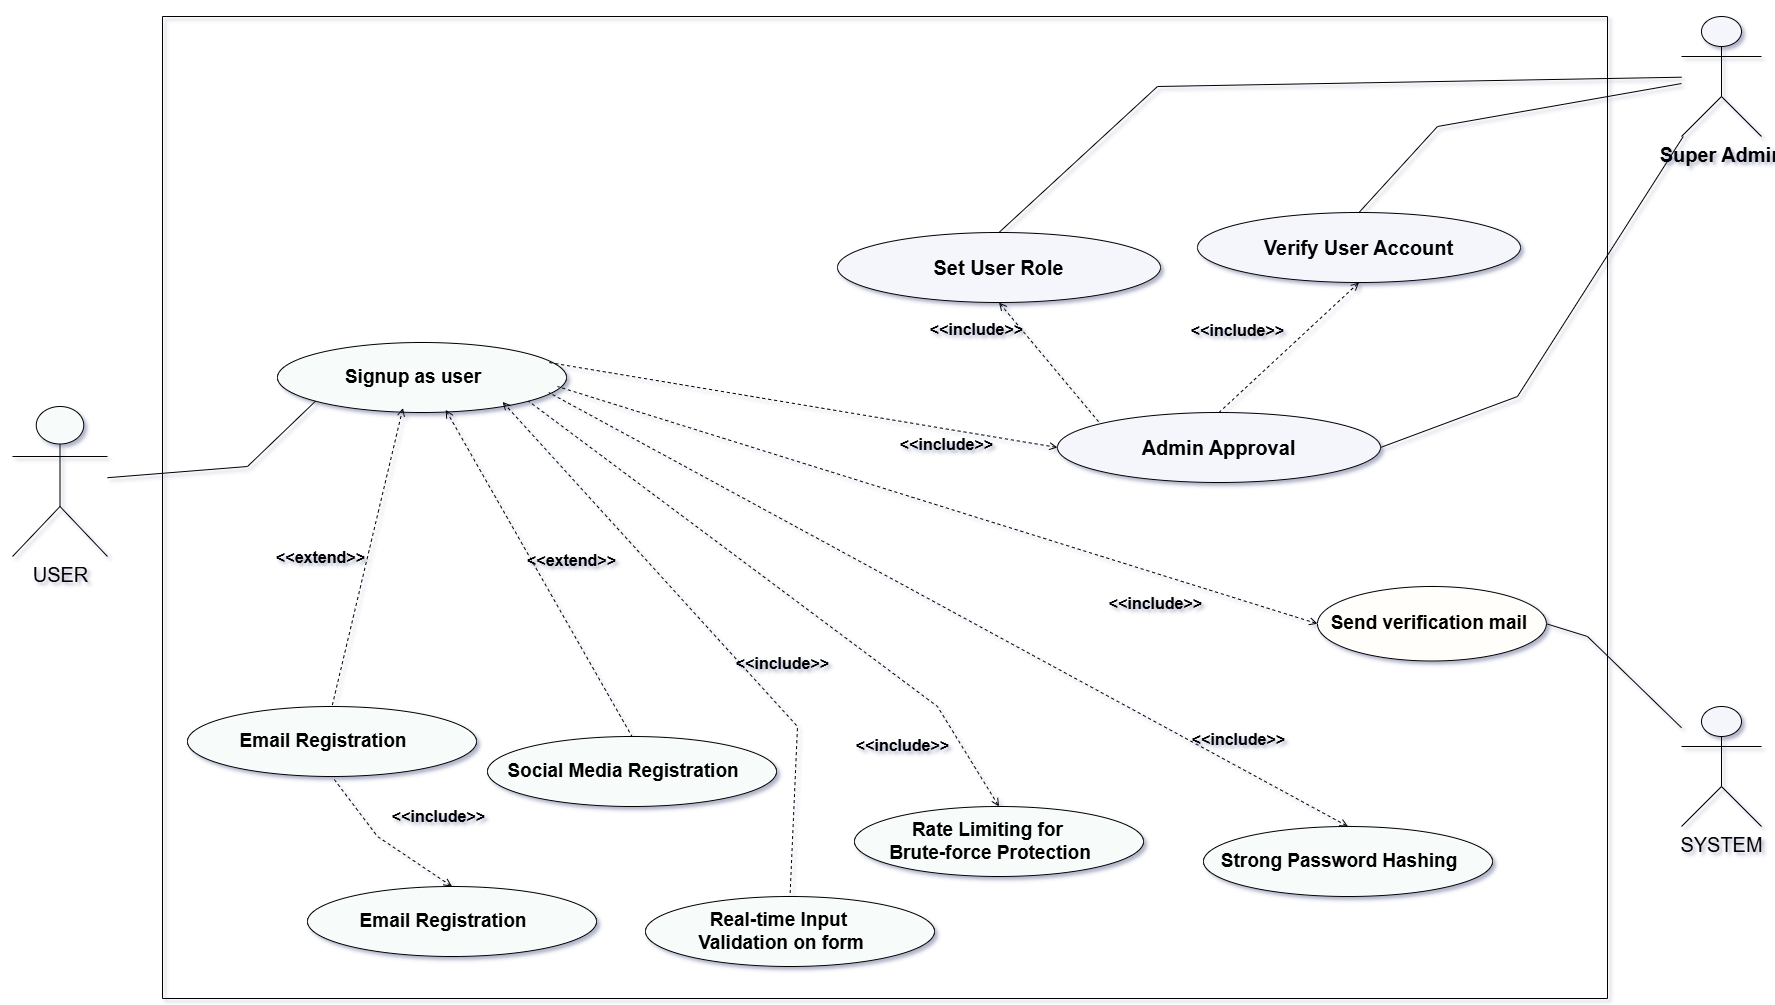
\includegraphics[width=1\textwidth]{images/diagram_de_case_d_utilisation_signup.png}
    \caption{Authentication Sign-up Use Case Diagram}
    \label{fig:signup-diagram}
\end{figure}

% \vspace{1cm}


The sign-up process includes user registration, role assignment, and account verification steps. During registration, users are categorized into one of the three user types: Super Admin, Admin, or Agent, with each type having different permissions and access levels within the system.

% Additional sections for subsequent sprints will be added later 